% Options for packages loaded elsewhere
\PassOptionsToPackage{unicode}{hyperref}
\PassOptionsToPackage{hyphens}{url}
\PassOptionsToPackage{dvipsnames,svgnames,x11names}{xcolor}
%
\documentclass[
]{article}
\usepackage{amsmath,amssymb}
\usepackage{iftex}
\ifPDFTeX
  \usepackage[T1]{fontenc}
  \usepackage[utf8]{inputenc}
  \usepackage{textcomp} % provide euro and other symbols
\else % if luatex or xetex
  \usepackage{unicode-math} % this also loads fontspec
  \defaultfontfeatures{Scale=MatchLowercase}
  \defaultfontfeatures[\rmfamily]{Ligatures=TeX,Scale=1}
\fi
\usepackage{lmodern}
\ifPDFTeX\else
  % xetex/luatex font selection
\fi
% Use upquote if available, for straight quotes in verbatim environments
\IfFileExists{upquote.sty}{\usepackage{upquote}}{}
\IfFileExists{microtype.sty}{% use microtype if available
  \usepackage[]{microtype}
  \UseMicrotypeSet[protrusion]{basicmath} % disable protrusion for tt fonts
}{}
\makeatletter
\@ifundefined{KOMAClassName}{% if non-KOMA class
  \IfFileExists{parskip.sty}{%
    \usepackage{parskip}
  }{% else
    \setlength{\parindent}{0pt}
    \setlength{\parskip}{6pt plus 2pt minus 1pt}}
}{% if KOMA class
  \KOMAoptions{parskip=half}}
\makeatother
\usepackage{xcolor}
\usepackage[margin=1in]{geometry}
\usepackage{color}
\usepackage{fancyvrb}
\newcommand{\VerbBar}{|}
\newcommand{\VERB}{\Verb[commandchars=\\\{\}]}
\DefineVerbatimEnvironment{Highlighting}{Verbatim}{commandchars=\\\{\}}
% Add ',fontsize=\small' for more characters per line
\usepackage{framed}
\definecolor{shadecolor}{RGB}{248,248,248}
\newenvironment{Shaded}{\begin{snugshade}}{\end{snugshade}}
\newcommand{\AlertTok}[1]{\textcolor[rgb]{0.94,0.16,0.16}{#1}}
\newcommand{\AnnotationTok}[1]{\textcolor[rgb]{0.56,0.35,0.01}{\textbf{\textit{#1}}}}
\newcommand{\AttributeTok}[1]{\textcolor[rgb]{0.13,0.29,0.53}{#1}}
\newcommand{\BaseNTok}[1]{\textcolor[rgb]{0.00,0.00,0.81}{#1}}
\newcommand{\BuiltInTok}[1]{#1}
\newcommand{\CharTok}[1]{\textcolor[rgb]{0.31,0.60,0.02}{#1}}
\newcommand{\CommentTok}[1]{\textcolor[rgb]{0.56,0.35,0.01}{\textit{#1}}}
\newcommand{\CommentVarTok}[1]{\textcolor[rgb]{0.56,0.35,0.01}{\textbf{\textit{#1}}}}
\newcommand{\ConstantTok}[1]{\textcolor[rgb]{0.56,0.35,0.01}{#1}}
\newcommand{\ControlFlowTok}[1]{\textcolor[rgb]{0.13,0.29,0.53}{\textbf{#1}}}
\newcommand{\DataTypeTok}[1]{\textcolor[rgb]{0.13,0.29,0.53}{#1}}
\newcommand{\DecValTok}[1]{\textcolor[rgb]{0.00,0.00,0.81}{#1}}
\newcommand{\DocumentationTok}[1]{\textcolor[rgb]{0.56,0.35,0.01}{\textbf{\textit{#1}}}}
\newcommand{\ErrorTok}[1]{\textcolor[rgb]{0.64,0.00,0.00}{\textbf{#1}}}
\newcommand{\ExtensionTok}[1]{#1}
\newcommand{\FloatTok}[1]{\textcolor[rgb]{0.00,0.00,0.81}{#1}}
\newcommand{\FunctionTok}[1]{\textcolor[rgb]{0.13,0.29,0.53}{\textbf{#1}}}
\newcommand{\ImportTok}[1]{#1}
\newcommand{\InformationTok}[1]{\textcolor[rgb]{0.56,0.35,0.01}{\textbf{\textit{#1}}}}
\newcommand{\KeywordTok}[1]{\textcolor[rgb]{0.13,0.29,0.53}{\textbf{#1}}}
\newcommand{\NormalTok}[1]{#1}
\newcommand{\OperatorTok}[1]{\textcolor[rgb]{0.81,0.36,0.00}{\textbf{#1}}}
\newcommand{\OtherTok}[1]{\textcolor[rgb]{0.56,0.35,0.01}{#1}}
\newcommand{\PreprocessorTok}[1]{\textcolor[rgb]{0.56,0.35,0.01}{\textit{#1}}}
\newcommand{\RegionMarkerTok}[1]{#1}
\newcommand{\SpecialCharTok}[1]{\textcolor[rgb]{0.81,0.36,0.00}{\textbf{#1}}}
\newcommand{\SpecialStringTok}[1]{\textcolor[rgb]{0.31,0.60,0.02}{#1}}
\newcommand{\StringTok}[1]{\textcolor[rgb]{0.31,0.60,0.02}{#1}}
\newcommand{\VariableTok}[1]{\textcolor[rgb]{0.00,0.00,0.00}{#1}}
\newcommand{\VerbatimStringTok}[1]{\textcolor[rgb]{0.31,0.60,0.02}{#1}}
\newcommand{\WarningTok}[1]{\textcolor[rgb]{0.56,0.35,0.01}{\textbf{\textit{#1}}}}
\usepackage{graphicx}
\makeatletter
\def\maxwidth{\ifdim\Gin@nat@width>\linewidth\linewidth\else\Gin@nat@width\fi}
\def\maxheight{\ifdim\Gin@nat@height>\textheight\textheight\else\Gin@nat@height\fi}
\makeatother
% Scale images if necessary, so that they will not overflow the page
% margins by default, and it is still possible to overwrite the defaults
% using explicit options in \includegraphics[width, height, ...]{}
\setkeys{Gin}{width=\maxwidth,height=\maxheight,keepaspectratio}
% Set default figure placement to htbp
\makeatletter
\def\fps@figure{htbp}
\makeatother
\setlength{\emergencystretch}{3em} % prevent overfull lines
\providecommand{\tightlist}{%
  \setlength{\itemsep}{0pt}\setlength{\parskip}{0pt}}
\setcounter{secnumdepth}{-\maxdimen} % remove section numbering
\ifLuaTeX
  \usepackage{selnolig}  % disable illegal ligatures
\fi
\IfFileExists{bookmark.sty}{\usepackage{bookmark}}{\usepackage{hyperref}}
\IfFileExists{xurl.sty}{\usepackage{xurl}}{} % add URL line breaks if available
\urlstyle{same}
\hypersetup{
  pdftitle={STAT 847: Final Project},
  colorlinks=true,
  linkcolor={Maroon},
  filecolor={Maroon},
  citecolor={Blue},
  urlcolor={blue},
  pdfcreator={LaTeX via pandoc}}

\title{STAT 847: Final Project}
\usepackage{etoolbox}
\makeatletter
\providecommand{\subtitle}[1]{% add subtitle to \maketitle
  \apptocmd{\@title}{\par {\large #1 \par}}{}{}
}
\makeatother
\subtitle{DUE: Friday April 19, 2024 by 11:59pm Eastern}
\author{}
\date{\vspace{-2.5em}}

\begin{document}
\maketitle

Your assignment must be submitted by the due date listed at the top of
this document, and it must be submitted electronically in .pdf format
via Crowdmark.

Total word count target is 1000 words, there are 100 marks.
Approximately 15 for each of 6 parts (if one part is extra large, it
will count for more points), and 10 points for presentation as a whole.
Use your visualization and writing skills, as well as your data science
skills.

Find a dataset we didn't cover in class, it has to be large enough with
enough features to complete the parts listed below. (Notice that 4 are
mandatory, 4 are optional)

\vspace{2cm}

\begin{enumerate}
\def\labelenumi{\arabic{enumi})}
\tightlist
\item
  \textbf{MUST BE INCLUDED} Describe and justify two different topics or
  approaches you might want to consider for this dataset and task. You
  don't have to use these tasks in the actual analysis.
\end{enumerate}

For this project, I will be analyzing the House Prices dataset from the
``KAGGLE GETTING STARTED PREDICTION COMPETITION,'' which includes 1460
observations (houses) and 81 variables suitable for explanatory analysis
or feature engineering. I plan to explore two key topics with this
dataset:

\begin{enumerate}
\def\labelenumi{\arabic{enumi}.}
\tightlist
\item
  \textbf{Identification of Key Features Influencing Home Prices}: I aim
  to pinpoint the variables that most significantly impact the pricing
  of a home. Understanding these key drivers will not only aid home
  developers in tailoring their constructions to meet market demands but
  will also enable them to command higher prices by emphasizing the
  features that prospective buyers value most.
\item
  \textbf{Home Price Prediction Model}: By using the identified
  important features, I will develop a predictive model for home prices.
  The model will be evaluated to ensure accuracy. This approach is
  particularly useful for various stakeholders. For realtors and
  investors, accurately predicting home prices helps in identifying
  whether homes are underpriced (indicating potential bargains) or
  overpriced (which could lead to prolonged market listings and
  decreased attractiveness).
\end{enumerate}

These approaches are not just academic exercises; they have practical
implications that could lead to more informed decision-making in the
real estate market. By leveraging data to identify and predict key
factors affecting home prices, stakeholders can optimize their
strategies to maximize returns and efficiency in the property market.

\vspace{2cm}

\newpage

\begin{enumerate}
\def\labelenumi{\arabic{enumi})}
\setcounter{enumi}{1}
\tightlist
\item
  \textbf{MUST BE INCLUDED} Give a ggpairs plot of what you think are
  the six most important variables. At least one must be categorical,
  and one continuous. Explain your choice of variables and the trends
  between them.
\end{enumerate}

\begin{Shaded}
\begin{Highlighting}[]
\FunctionTok{library}\NormalTok{(GGally)}

\NormalTok{Q2\_plot }\OtherTok{\textless{}{-}} \FunctionTok{ggpairs}\NormalTok{(Q2\_df)}

\NormalTok{Q2\_plot}
\end{Highlighting}
\end{Shaded}

\begin{figure}
\centering
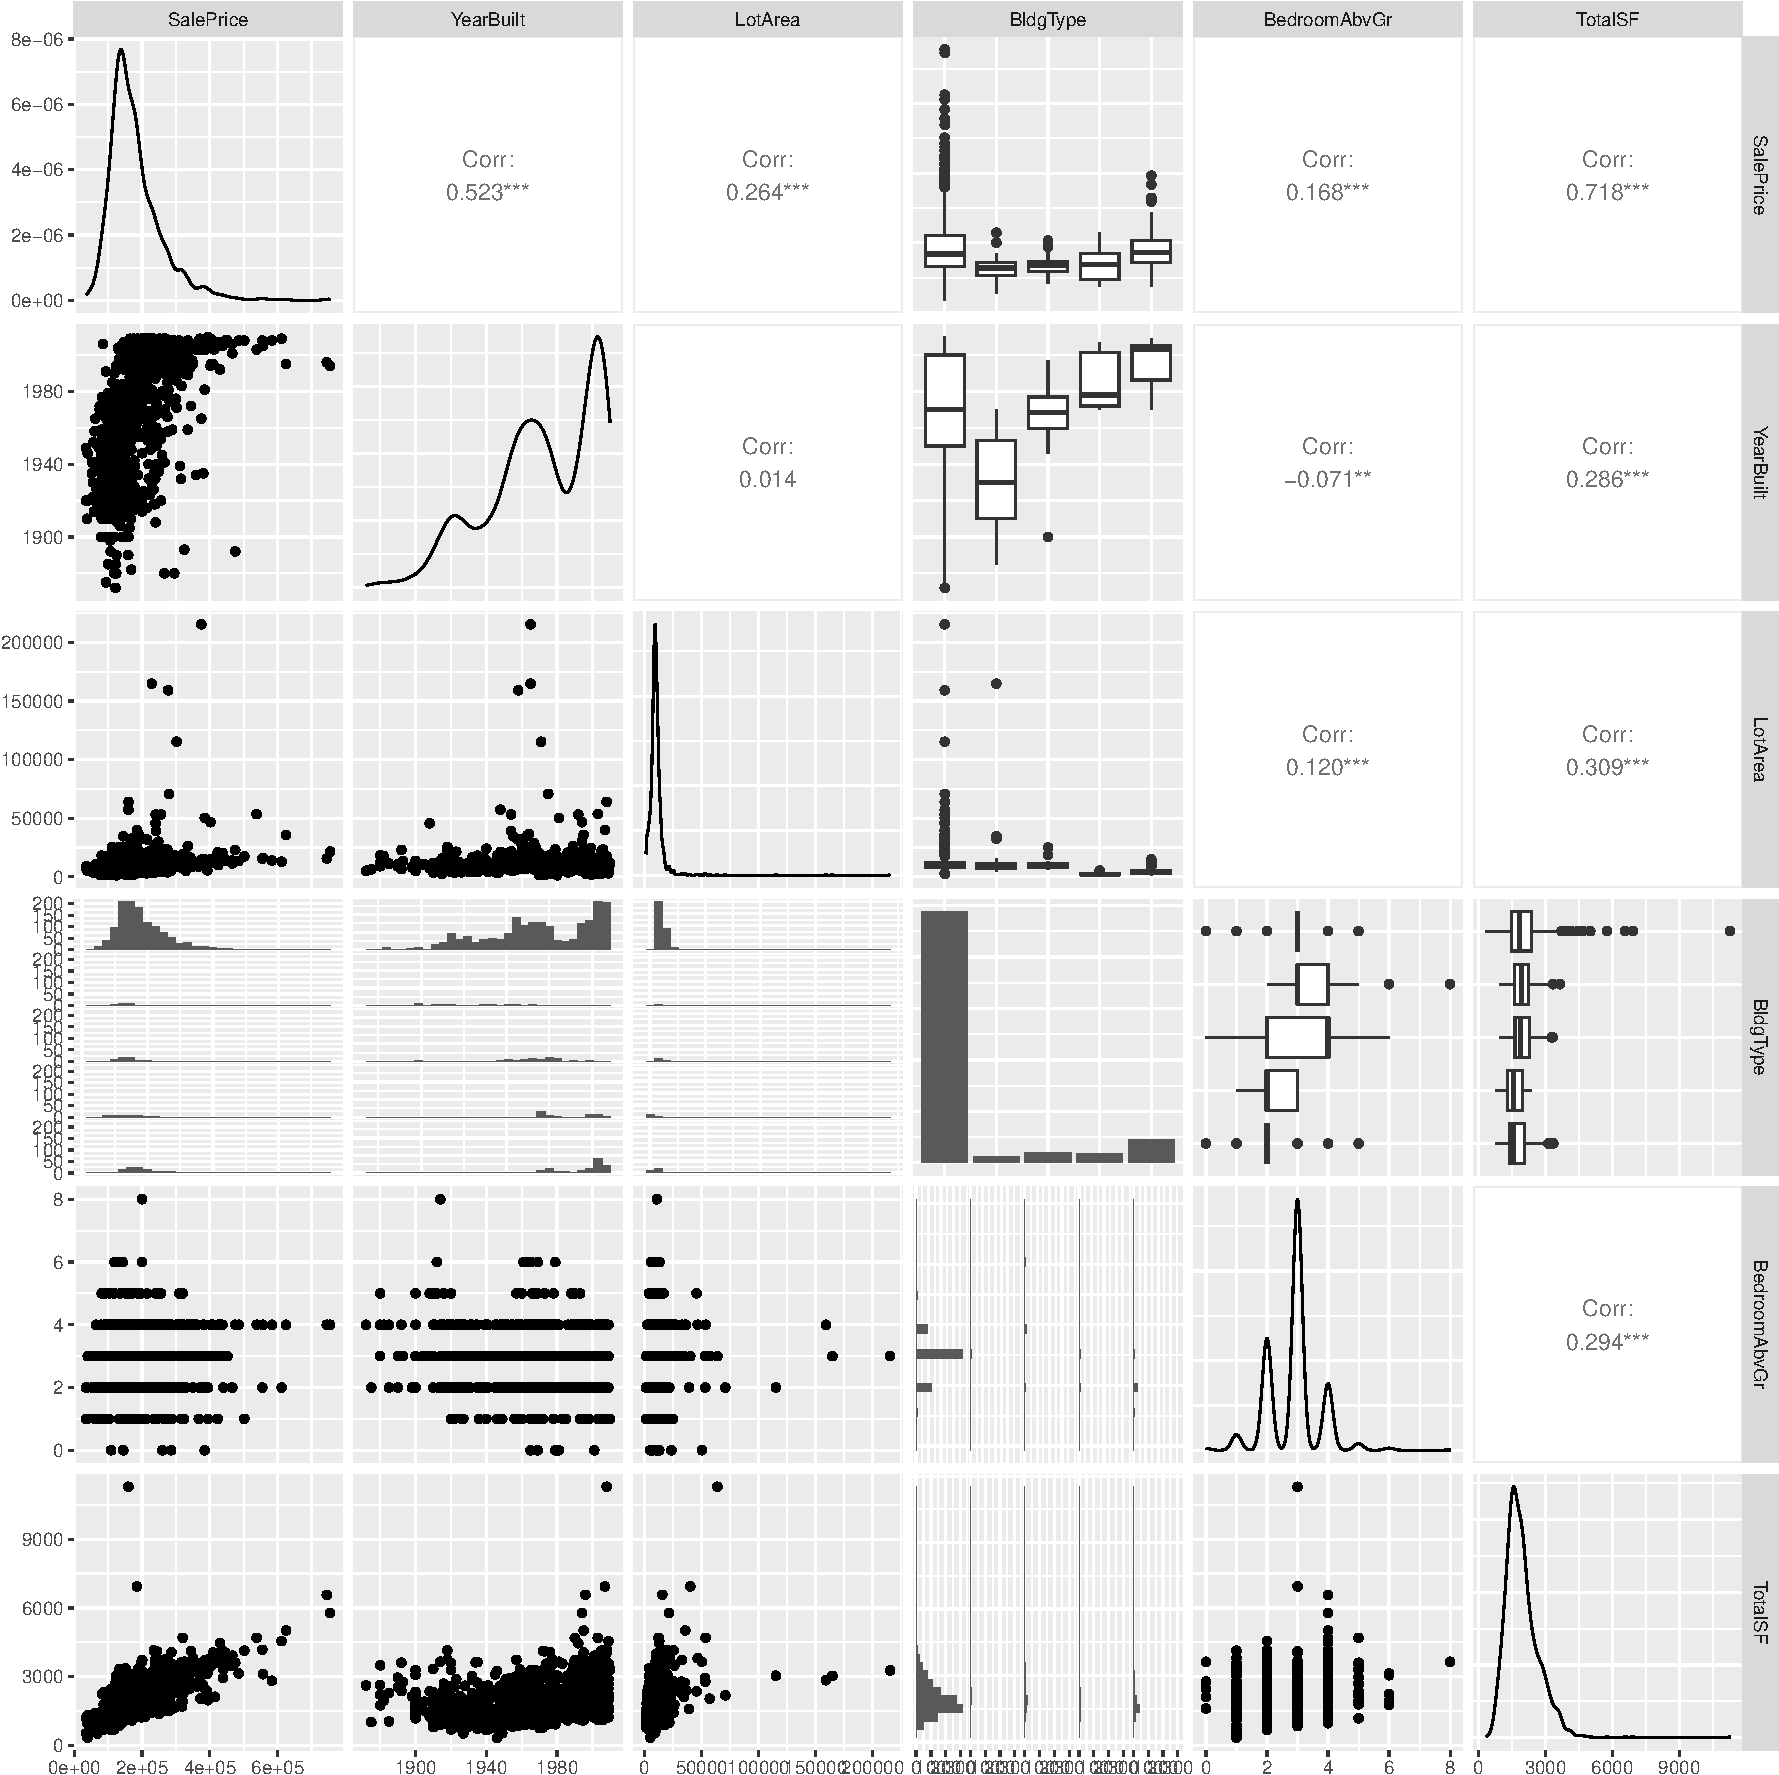
\includegraphics{STAT847_W24_Final_files/figure-latex/unnamed-chunk-7-1.pdf}
\caption{GGpairs plot of the 6 variables I believe are most important.}
\end{figure}

\newpage

For this exercise I chose the variables SalePrice, YearBuilt,
LotFrontage, LotArea, BldgType, BedroomAbvGr.

\begin{enumerate}
\def\labelenumi{\arabic{enumi}.}
\item
  \textbf{SalePrice}: This variable captures the price the home was sold
  for. This will be my dependant in my prediction model.
\item
  \textbf{YearBuilt}: The YearBuilt variable depicts the original
  construction date. This is important because housing has definately
  improved over time and so the construction date can be a predictor for
  the quality of the build.
\item
  \textbf{TotalSF}: I created this variable to capture the total square
  footage of the home by adding the square footage of the basement and
  the square footage of all home area above grade (above soil level). I
  believe this variable is important because typically bigger families
  need more home area and are willing to pay more for that so this can
  definately impact the house price.
\item
  \textbf{LotArea}: This varable captures the lot size in square feet.
  This is an important factor since the amount of area of a property
  could increase the value as the home square feet may not capture the
  amount of land in the transaction.
\item
  \textbf{BldgType}: The variable BldgType captures the type of
  dwelling:
\end{enumerate}

\begin{itemize}
\tightlist
\item
  1Fam: Single-family Detached\\
\item
  2FmCon Two-family Conversion; originally built as one-family dwelling
\item
  Duplx: Duplex
\item
  TwnhsE: Townhouse End Unit
\item
  TwnhsI: Townhouse Inside Unit
\end{itemize}

I chose this variable due to the type of house having a great impact on
the price. An example of this is that a duplex and a single family
detached could have the same square footage however since the duplex can
accomodate two families it could be worth more.

\begin{enumerate}
\def\labelenumi{\arabic{enumi}.}
\setcounter{enumi}{5}
\tightlist
\item
  \textbf{BedroomAbvGr}: The BedroomAbvGr variable captures the number
  of bedrooms above grade (does NOT include basement bedrooms). This
  variable is important because the number of bedrooms can be a deciding
  factor for a family on whether they will buy the house or not
  depending on whether it has enough rooms to accommodate their family.
\end{enumerate}

With regards to the relationships seen in between the variables in the
ggpairs plot. The first one that stuck out to me was the strong positive
correlation between Total square footage and Sale Price which makes
sense since individuals will pay more for a home with more square
footage.We observe a weak positive correlation between the number of
bedrooms above ground and the total square footage, this is certainly
due to the opportunity to build more bedrooms as the square footage
increases however its weak since theres only so many bedrooms that a
house can have before its too much. we see a weak positive correlation
between YearBuilt and total square footage which weeakly tells us that
over time homes have been increasing in size. We see little to no
correlation to lot area and year built with along with the last
correlation tells us that over time more home are being built with
square footage in mind over the lot area, which is an important factor
to look out for in my model. Im expecting now to see a high importance
on total square footage of a home which determined the switch to
prioritizing total square footage. Another interesting correlation is
the correlation between YearBuilt and sale price, we see a exponential
rise that over time is reaching a limit, i believe this is due to the
inflation of the dollar and the housing market reaching a peak around
2008 before the housing crisis then we see that the price levels off due
to the market crash.

\vspace{2cm}

\newpage

\begin{enumerate}
\def\labelenumi{\arabic{enumi})}
\setcounter{enumi}{2}
\tightlist
\item
  \textbf{MUST BE INCLUDED} Build a classification tree of one of the
  six variables from the last part as a function of the other five, and
  any other explanatory variables you think are necessary. Show code,
  explain reasoning, and show the tree as a simple (ugly) plot. Show the
  confusion matrix. Give two example predictions and follow them down
  the tree.
\end{enumerate}

For this question i will be adding the variables Fireplaces, GarageType,
PoolArea, SaleType, and remodel to the dataset. Fireplace is a count of
the number of fireplaces in the home, I am adding this variable since
personally I am a big fan of fireplaces and would need a fireplace in my
home for me to make the purchase. GarageType is a variable that captures
what type of garage the home has, again I am choosing to add this
variable due to me enjoying spending time in my garage working on my car
so I would like to see the impact the GarageType could have on a home.
PoolArea captures the area of a pool and is 0 if there is no pool, I am
adding this to see the impact a pool could have on a home, I am
expecting little to no impact. SaleType is a catagorical variable with
many factors however the two I am most interested in and most prominent
are WD: Warranty Deed - Conventional and New: Home just constructed and
sold. and finally remodel is a variable I created that checks if there
is a remodel date, if yes then the house was remodeled and it is a 1
else it is 0 so the variable captures if the house was remodeled after
being built or not.

I will create a classification tree to predict the number of bedrooms
above grade as a function of all the other variables in the dataset (all
the variables mentioned in Q2 plus the ones mentioned above).

\begin{Shaded}
\begin{Highlighting}[]
\NormalTok{Q3\_df }\OtherTok{\textless{}{-}}\NormalTok{ house\_df }\SpecialCharTok{\%\textgreater{}\%}
    \FunctionTok{select}\NormalTok{(SalePrice, YearBuilt, LotArea, BldgType,}
\NormalTok{        BedroomAbvGr, GrLivArea, BsmtFinSF1, Fireplaces,}
\NormalTok{        GarageType, PoolArea, SaleType, YearRemodAdd,}
\NormalTok{        YearBuilt) }\SpecialCharTok{\%\textgreater{}\%}
    \FunctionTok{mutate}\NormalTok{(}\AttributeTok{TotalSF =}\NormalTok{ BsmtFinSF1 }\SpecialCharTok{+}\NormalTok{ GrLivArea, }\AttributeTok{remodel =} \FunctionTok{if\_else}\NormalTok{(YearRemodAdd }\SpecialCharTok{!=}
\NormalTok{        YearBuilt, }\DecValTok{1}\NormalTok{, }\DecValTok{0}\NormalTok{), }\AttributeTok{GarageType =} \FunctionTok{if\_else}\NormalTok{(}\FunctionTok{is.na}\NormalTok{(GarageType),}
        \StringTok{"NoGarage"}\NormalTok{, GarageType)) }\SpecialCharTok{\%\textgreater{}\%}
    \FunctionTok{select}\NormalTok{(}\SpecialCharTok{{-}}\NormalTok{GrLivArea, }\SpecialCharTok{{-}}\NormalTok{BsmtFinSF1, }\SpecialCharTok{{-}}\NormalTok{YearRemodAdd)}

\NormalTok{Q3\_df}\SpecialCharTok{$}\NormalTok{BedroomAbvGr }\OtherTok{\textless{}{-}} \FunctionTok{as.factor}\NormalTok{(Q3\_df}\SpecialCharTok{$}\NormalTok{BedroomAbvGr)}
\end{Highlighting}
\end{Shaded}

\newpage

\begin{Shaded}
\begin{Highlighting}[]
\NormalTok{tree\_model }\OtherTok{\textless{}{-}} \FunctionTok{tree}\NormalTok{(BedroomAbvGr }\SpecialCharTok{\textasciitilde{}}\NormalTok{ ., }\AttributeTok{data =}\NormalTok{ Q3\_df)}

\CommentTok{\# Plot the tree}
\FunctionTok{plot}\NormalTok{(tree\_model, }\AttributeTok{uniform =} \ConstantTok{TRUE}\NormalTok{, }\AttributeTok{main =} \StringTok{"Classification tree"}\NormalTok{)}
\FunctionTok{text}\NormalTok{(tree\_model, }\AttributeTok{use.n =} \ConstantTok{TRUE}\NormalTok{, }\AttributeTok{pretty =} \DecValTok{0}\NormalTok{)}
\end{Highlighting}
\end{Shaded}

\begin{figure}
\centering
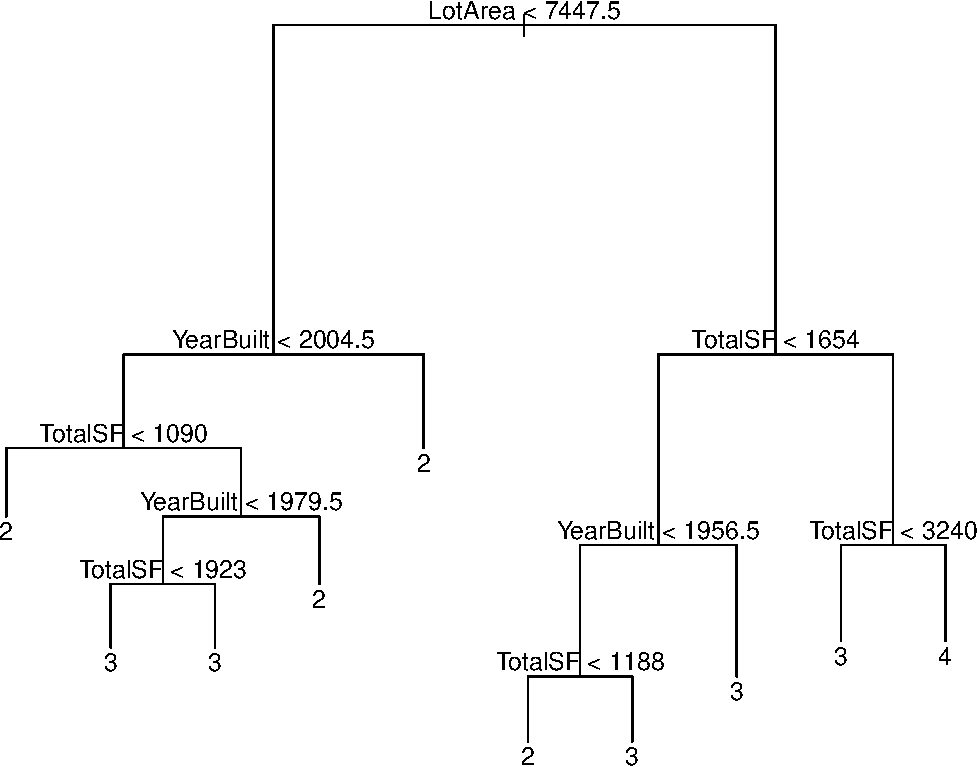
\includegraphics{STAT847_W24_Final_files/figure-latex/unnamed-chunk-9-1.pdf}
\caption{Simple(ugly) plot of the classification tree created to predict
number of bedrooms above grade(above soil level).}
\end{figure}

\newpage

\begin{Shaded}
\begin{Highlighting}[]
\NormalTok{plt }\OtherTok{\textless{}{-}} \FunctionTok{as.data.frame}\NormalTok{(confusion\_matrix}\SpecialCharTok{$}\NormalTok{table)}
\NormalTok{plt}\SpecialCharTok{$}\NormalTok{Prediction }\OtherTok{\textless{}{-}} \FunctionTok{factor}\NormalTok{(plt}\SpecialCharTok{$}\NormalTok{Prediction, }\AttributeTok{levels =} \FunctionTok{rev}\NormalTok{(}\FunctionTok{levels}\NormalTok{(plt}\SpecialCharTok{$}\NormalTok{Prediction)))}

\FunctionTok{ggplot}\NormalTok{(plt, }\FunctionTok{aes}\NormalTok{(}\AttributeTok{x =}\NormalTok{ Reference, }\AttributeTok{y =}\NormalTok{ Prediction,}
    \AttributeTok{fill =}\NormalTok{ Freq)) }\SpecialCharTok{+} \FunctionTok{geom\_tile}\NormalTok{() }\SpecialCharTok{+} \FunctionTok{geom\_text}\NormalTok{(}\FunctionTok{aes}\NormalTok{(}\AttributeTok{label =}\NormalTok{ Freq),}
    \AttributeTok{vjust =} \DecValTok{1}\NormalTok{) }\SpecialCharTok{+} \FunctionTok{scale\_fill\_gradient}\NormalTok{(}\AttributeTok{low =} \StringTok{"white"}\NormalTok{,}
    \AttributeTok{high =} \StringTok{"\#009194"}\NormalTok{) }\SpecialCharTok{+} \FunctionTok{labs}\NormalTok{(}\AttributeTok{x =} \StringTok{"Reference"}\NormalTok{,}
    \AttributeTok{y =} \StringTok{"Prediction"}\NormalTok{, }\AttributeTok{title =} \StringTok{"Confusion Matrix Visualization"}\NormalTok{) }\SpecialCharTok{+}
    \FunctionTok{scale\_x\_discrete}\NormalTok{(}\AttributeTok{labels =} \FunctionTok{c}\NormalTok{(}\StringTok{"0"}\NormalTok{, }\StringTok{"1"}\NormalTok{, }\StringTok{"2"}\NormalTok{,}
        \StringTok{"3"}\NormalTok{, }\StringTok{"4"}\NormalTok{, }\StringTok{"5"}\NormalTok{, }\StringTok{"6"}\NormalTok{, }\StringTok{"8"}\NormalTok{)) }\SpecialCharTok{+} \FunctionTok{scale\_y\_discrete}\NormalTok{(}\AttributeTok{labels =} \FunctionTok{c}\NormalTok{(}\StringTok{"8"}\NormalTok{,}
    \StringTok{"6"}\NormalTok{, }\StringTok{"5"}\NormalTok{, }\StringTok{"4"}\NormalTok{, }\StringTok{"3"}\NormalTok{, }\StringTok{"2"}\NormalTok{, }\StringTok{"1"}\NormalTok{, }\StringTok{"0"}\NormalTok{))}
\end{Highlighting}
\end{Shaded}

\begin{figure}
\centering
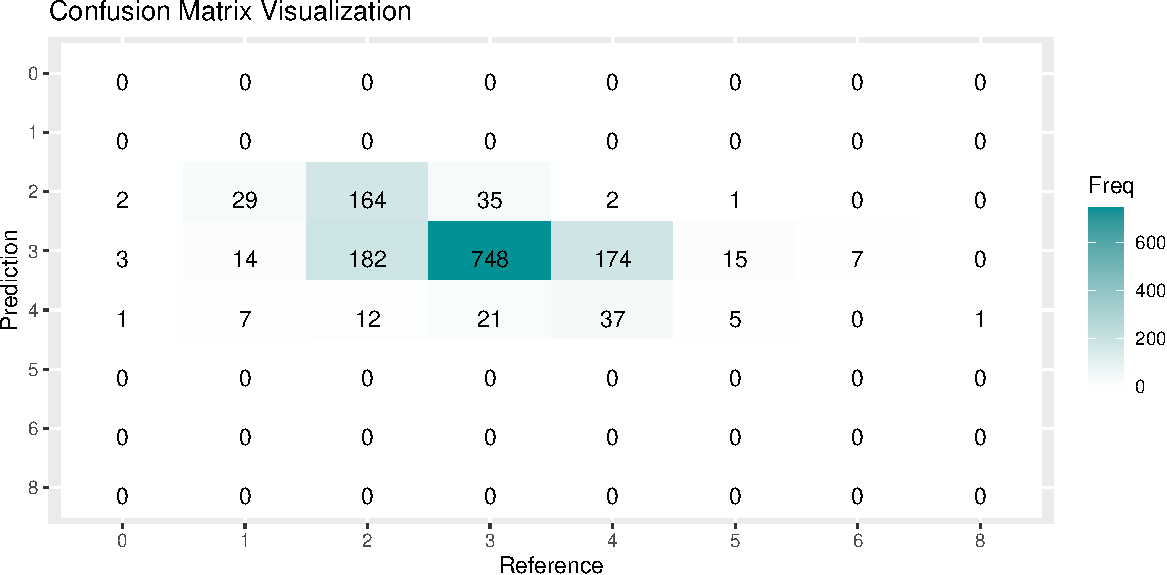
\includegraphics{STAT847_W24_Final_files/figure-latex/unnamed-chunk-11-1.pdf}
\caption{Confusion matrix plot of the predictions made on the housing
dataset.}
\end{figure}

\begin{table}[!h]
\centering
\caption{Sample Real Estate Data}
\tiny
\begin{tabular}{|c|c|c|c|c|c|c|c|c|c|c|}
\hline
\textbf{SalePrice} & \textbf{YearBuilt} & \textbf{LotArea} & \textbf{BldgType} & \textbf{BedroomAbvGr} & \textbf{Fireplaces} & \textbf{GarageType} & \textbf{PoolArea} & \textbf{SaleType} & \textbf{TotalSF} & \textbf{Remodel} \\
\hline
90000 & 1967 & 10791 & Duplex & 2 & 0 & CarPort & 0 & WD & 1296 & 0 \\
\hline
118000 & 1939 & 7420 & 2fmCon & 2 & 2 & Attchd & 0 & WD & 1928 & 1 \\
\hline
\end{tabular}
\end{table}

For the first row in the 2 example predictions we first see that the
LotArea is 10791 which is greater than 7447.5 therefore since the first
decision is false we follow the left tree. Next we see that the
YearBuilt is 1967 which is less than 2004.5 therefore that decision tree
is true and we follow the right tree leading us to the correct
prediction that the number of bedrooms above grade is 2.

For the second row in the 2 example prediction we see that the LotArea
is 7420 which is less than 7447.5 since this is true we follow the right
tree. Next we see that the TotalSF is 1928 which is greater than 1654
making this decision false so we follow the left tree, next we see tha
the YearBuilt less than 1956.5 is true therefore we incorrectly predict
that this home has 3 above grade bedrooms when in reality it only has 2.

See the following two pages for visual depictions of the predictions.

\begin{figure}
\centering
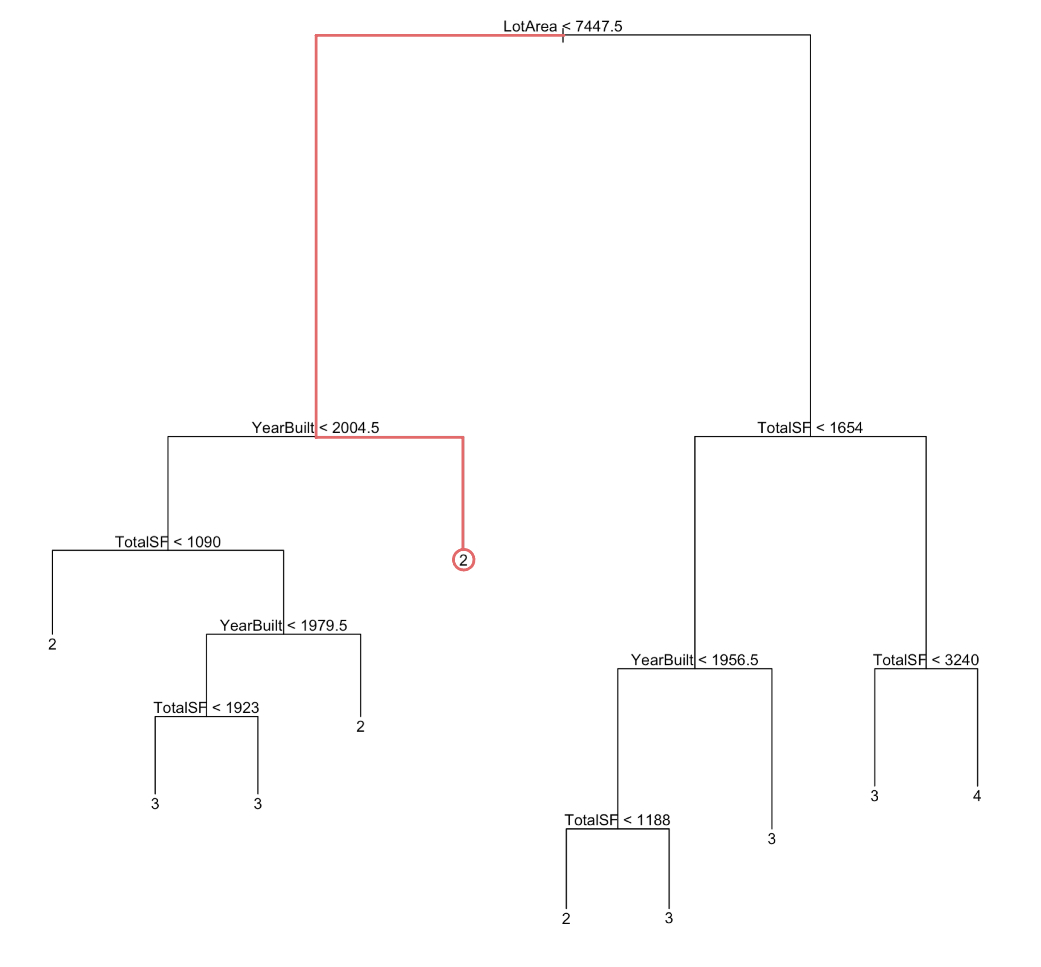
\includegraphics{/Users/andrew/Downloads/UW courses/STAT 847/Final/Q3_row2.jpeg}
\caption{A visual depiction of the tree classification for the first row
of the sample real estate data from Table 1.}
\end{figure}

\begin{figure}
\centering
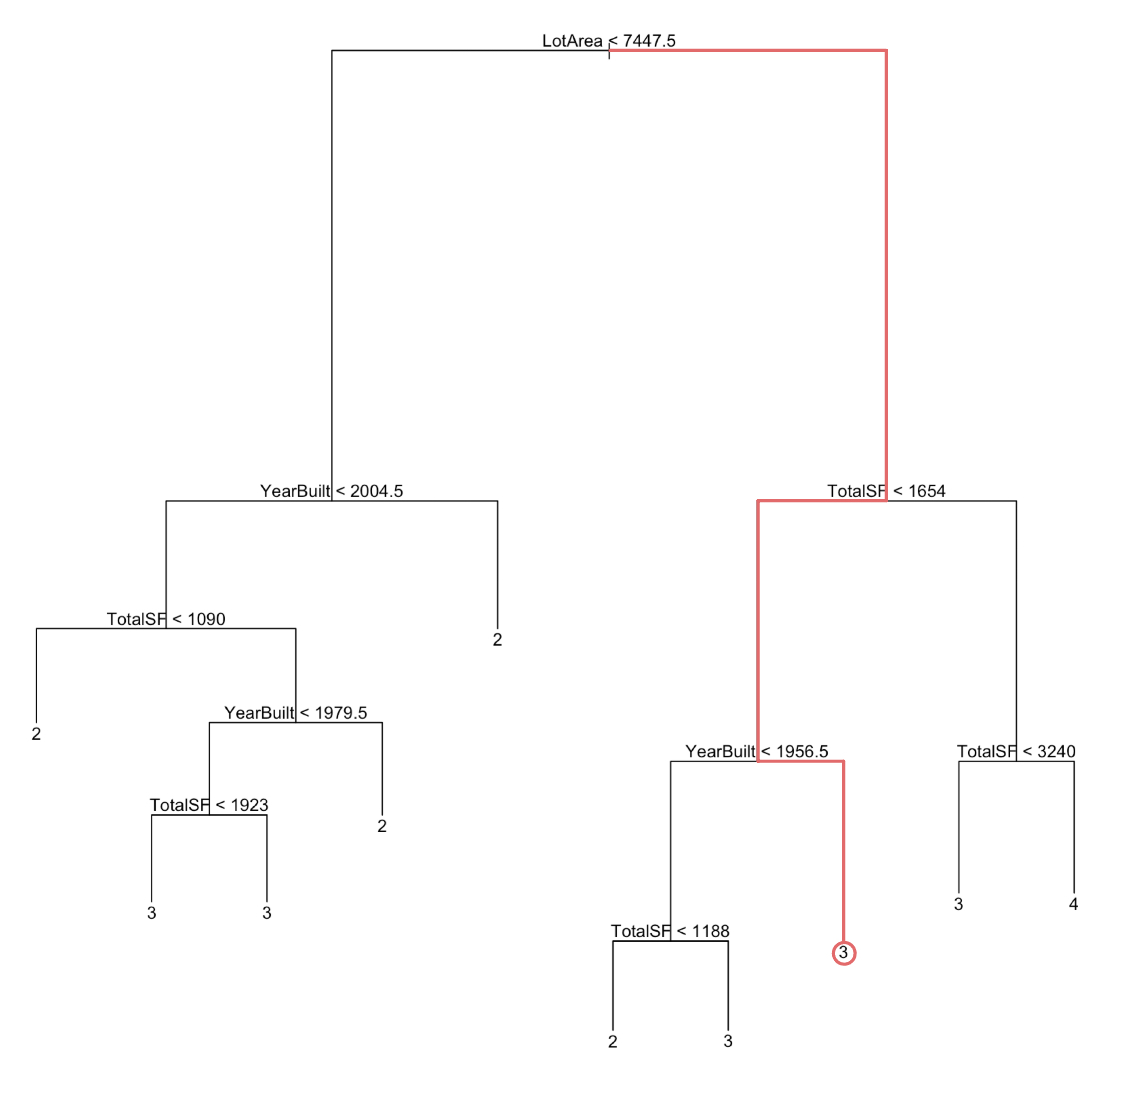
\includegraphics{/Users/andrew/Downloads/UW courses/STAT 847/Final/Q3_row1.jpeg}
\caption{A visual depiction of the tree classification for the second
row of the sample real estate data from Table 1.}
\end{figure}

\newpage

\begin{enumerate}
\def\labelenumi{\arabic{enumi})}
\setcounter{enumi}{3}
\tightlist
\item
  \textbf{MUST BE INCLUDED} Build another model using one of the
  continuous variables from your six most important. This time use your
  model selection and dimension reduction tools, and include at least
  one non-linear term.
\end{enumerate}

\begin{Shaded}
\begin{Highlighting}[]
\NormalTok{Q4\_df }\OtherTok{\textless{}{-}}\NormalTok{ Q3\_df }\SpecialCharTok{\%\textgreater{}\%}
    \FunctionTok{mutate}\NormalTok{(}\AttributeTok{TotalSF\_squared =}\NormalTok{ TotalSF}\SpecialCharTok{\^{}}\DecValTok{2}\NormalTok{)}
\end{Highlighting}
\end{Shaded}

\begin{Shaded}
\begin{Highlighting}[]
\FunctionTok{set.seed}\NormalTok{(}\DecValTok{21108082}\NormalTok{)}

\NormalTok{prelim\_rf }\OtherTok{\textless{}{-}} \FunctionTok{randomForest}\NormalTok{(SalePrice }\SpecialCharTok{\textasciitilde{}}\NormalTok{ ., }\AttributeTok{data =}\NormalTok{ Q4\_df,}
    \AttributeTok{ntree =} \DecValTok{100}\NormalTok{)}

\NormalTok{var\_importance }\OtherTok{\textless{}{-}} \FunctionTok{importance}\NormalTok{(prelim\_rf)}

\NormalTok{importance\_df }\OtherTok{\textless{}{-}} \FunctionTok{as.data.frame}\NormalTok{(var\_importance)}
\NormalTok{importance\_df}\SpecialCharTok{$}\NormalTok{Variable }\OtherTok{\textless{}{-}} \FunctionTok{rownames}\NormalTok{(importance\_df)}

\NormalTok{importance\_df }\OtherTok{\textless{}{-}}\NormalTok{ importance\_df }\SpecialCharTok{\%\textgreater{}\%}
    \FunctionTok{select}\NormalTok{(Variable, IncNodePurity) }\SpecialCharTok{\%\textgreater{}\%}
    \FunctionTok{arrange}\NormalTok{(}\FunctionTok{desc}\NormalTok{(IncNodePurity))}

\FunctionTok{ggplot}\NormalTok{(importance\_df, }\FunctionTok{aes}\NormalTok{(}\AttributeTok{x =} \FunctionTok{reorder}\NormalTok{(Variable,}
\NormalTok{    IncNodePurity), }\AttributeTok{y =}\NormalTok{ IncNodePurity)) }\SpecialCharTok{+} \FunctionTok{geom\_bar}\NormalTok{(}\AttributeTok{stat =} \StringTok{"identity"}\NormalTok{,}
    \AttributeTok{fill =} \StringTok{"red"}\NormalTok{) }\SpecialCharTok{+} \FunctionTok{coord\_flip}\NormalTok{() }\SpecialCharTok{+} \FunctionTok{labs}\NormalTok{(}\AttributeTok{x =} \StringTok{"Variable"}\NormalTok{,}
    \AttributeTok{y =} \StringTok{"Importance (Node Impurity)"}\NormalTok{, }\AttributeTok{title =} \StringTok{"Variable Importance Plot"}\NormalTok{) }\SpecialCharTok{+}
    \FunctionTok{theme\_minimal}\NormalTok{()}
\end{Highlighting}
\end{Shaded}

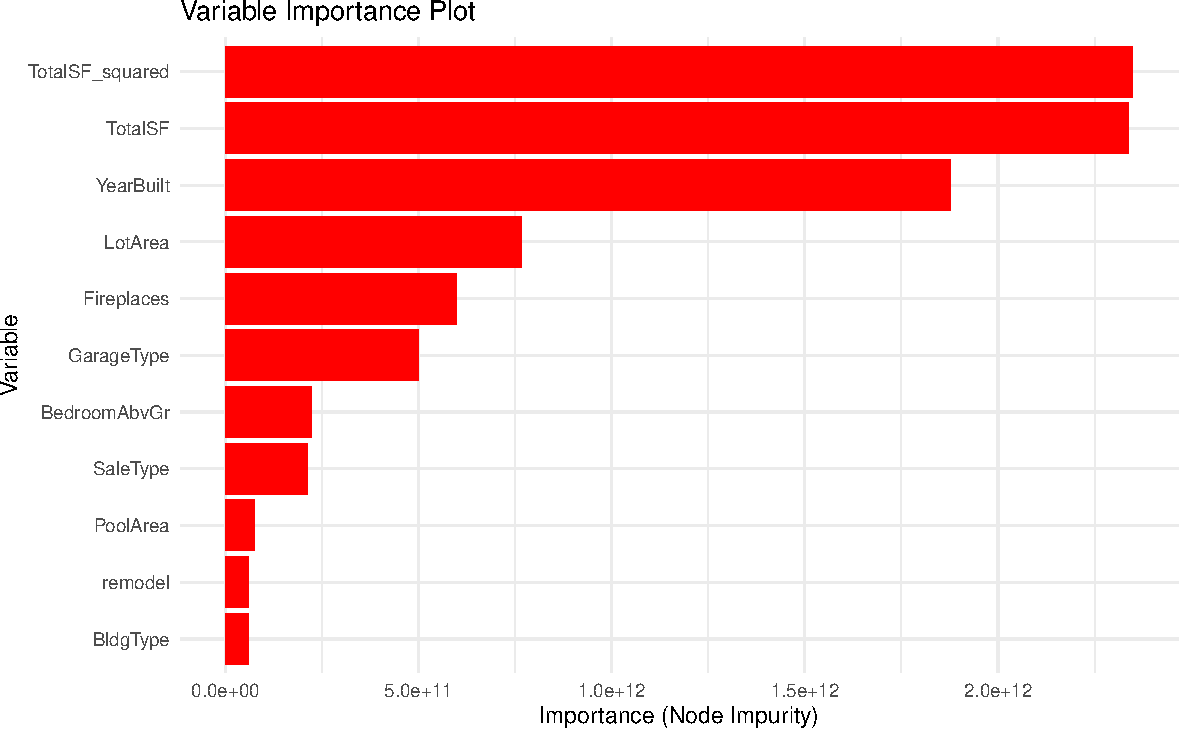
\includegraphics{STAT847_W24_Final_files/figure-latex/unnamed-chunk-15-1.pdf}
\newpage

\begin{Shaded}
\begin{Highlighting}[]
\FunctionTok{set.seed}\NormalTok{(}\DecValTok{21108082}\NormalTok{)}
\NormalTok{final\_rf }\OtherTok{\textless{}{-}} \FunctionTok{randomForest}\NormalTok{(SalePrice }\SpecialCharTok{\textasciitilde{}}\NormalTok{ TotalSF }\SpecialCharTok{+}
\NormalTok{    TotalSF\_squared }\SpecialCharTok{+}\NormalTok{ YearBuilt }\SpecialCharTok{+}\NormalTok{ LotArea }\SpecialCharTok{+}\NormalTok{ BedroomAbvGr }\SpecialCharTok{+}
\NormalTok{    GarageType, }\AttributeTok{data =}\NormalTok{ Q4\_df, }\AttributeTok{ntree =} \DecValTok{500}\NormalTok{)}

\NormalTok{reprtree}\SpecialCharTok{:::}\FunctionTok{plot.getTree}\NormalTok{(final\_rf)}
\end{Highlighting}
\end{Shaded}

\begin{verbatim}
## Registered S3 method overwritten by 'reprtree':
##   method    from
##   text.tree tree
\end{verbatim}

\begin{verbatim}
## Loading required package: plotrix
\end{verbatim}

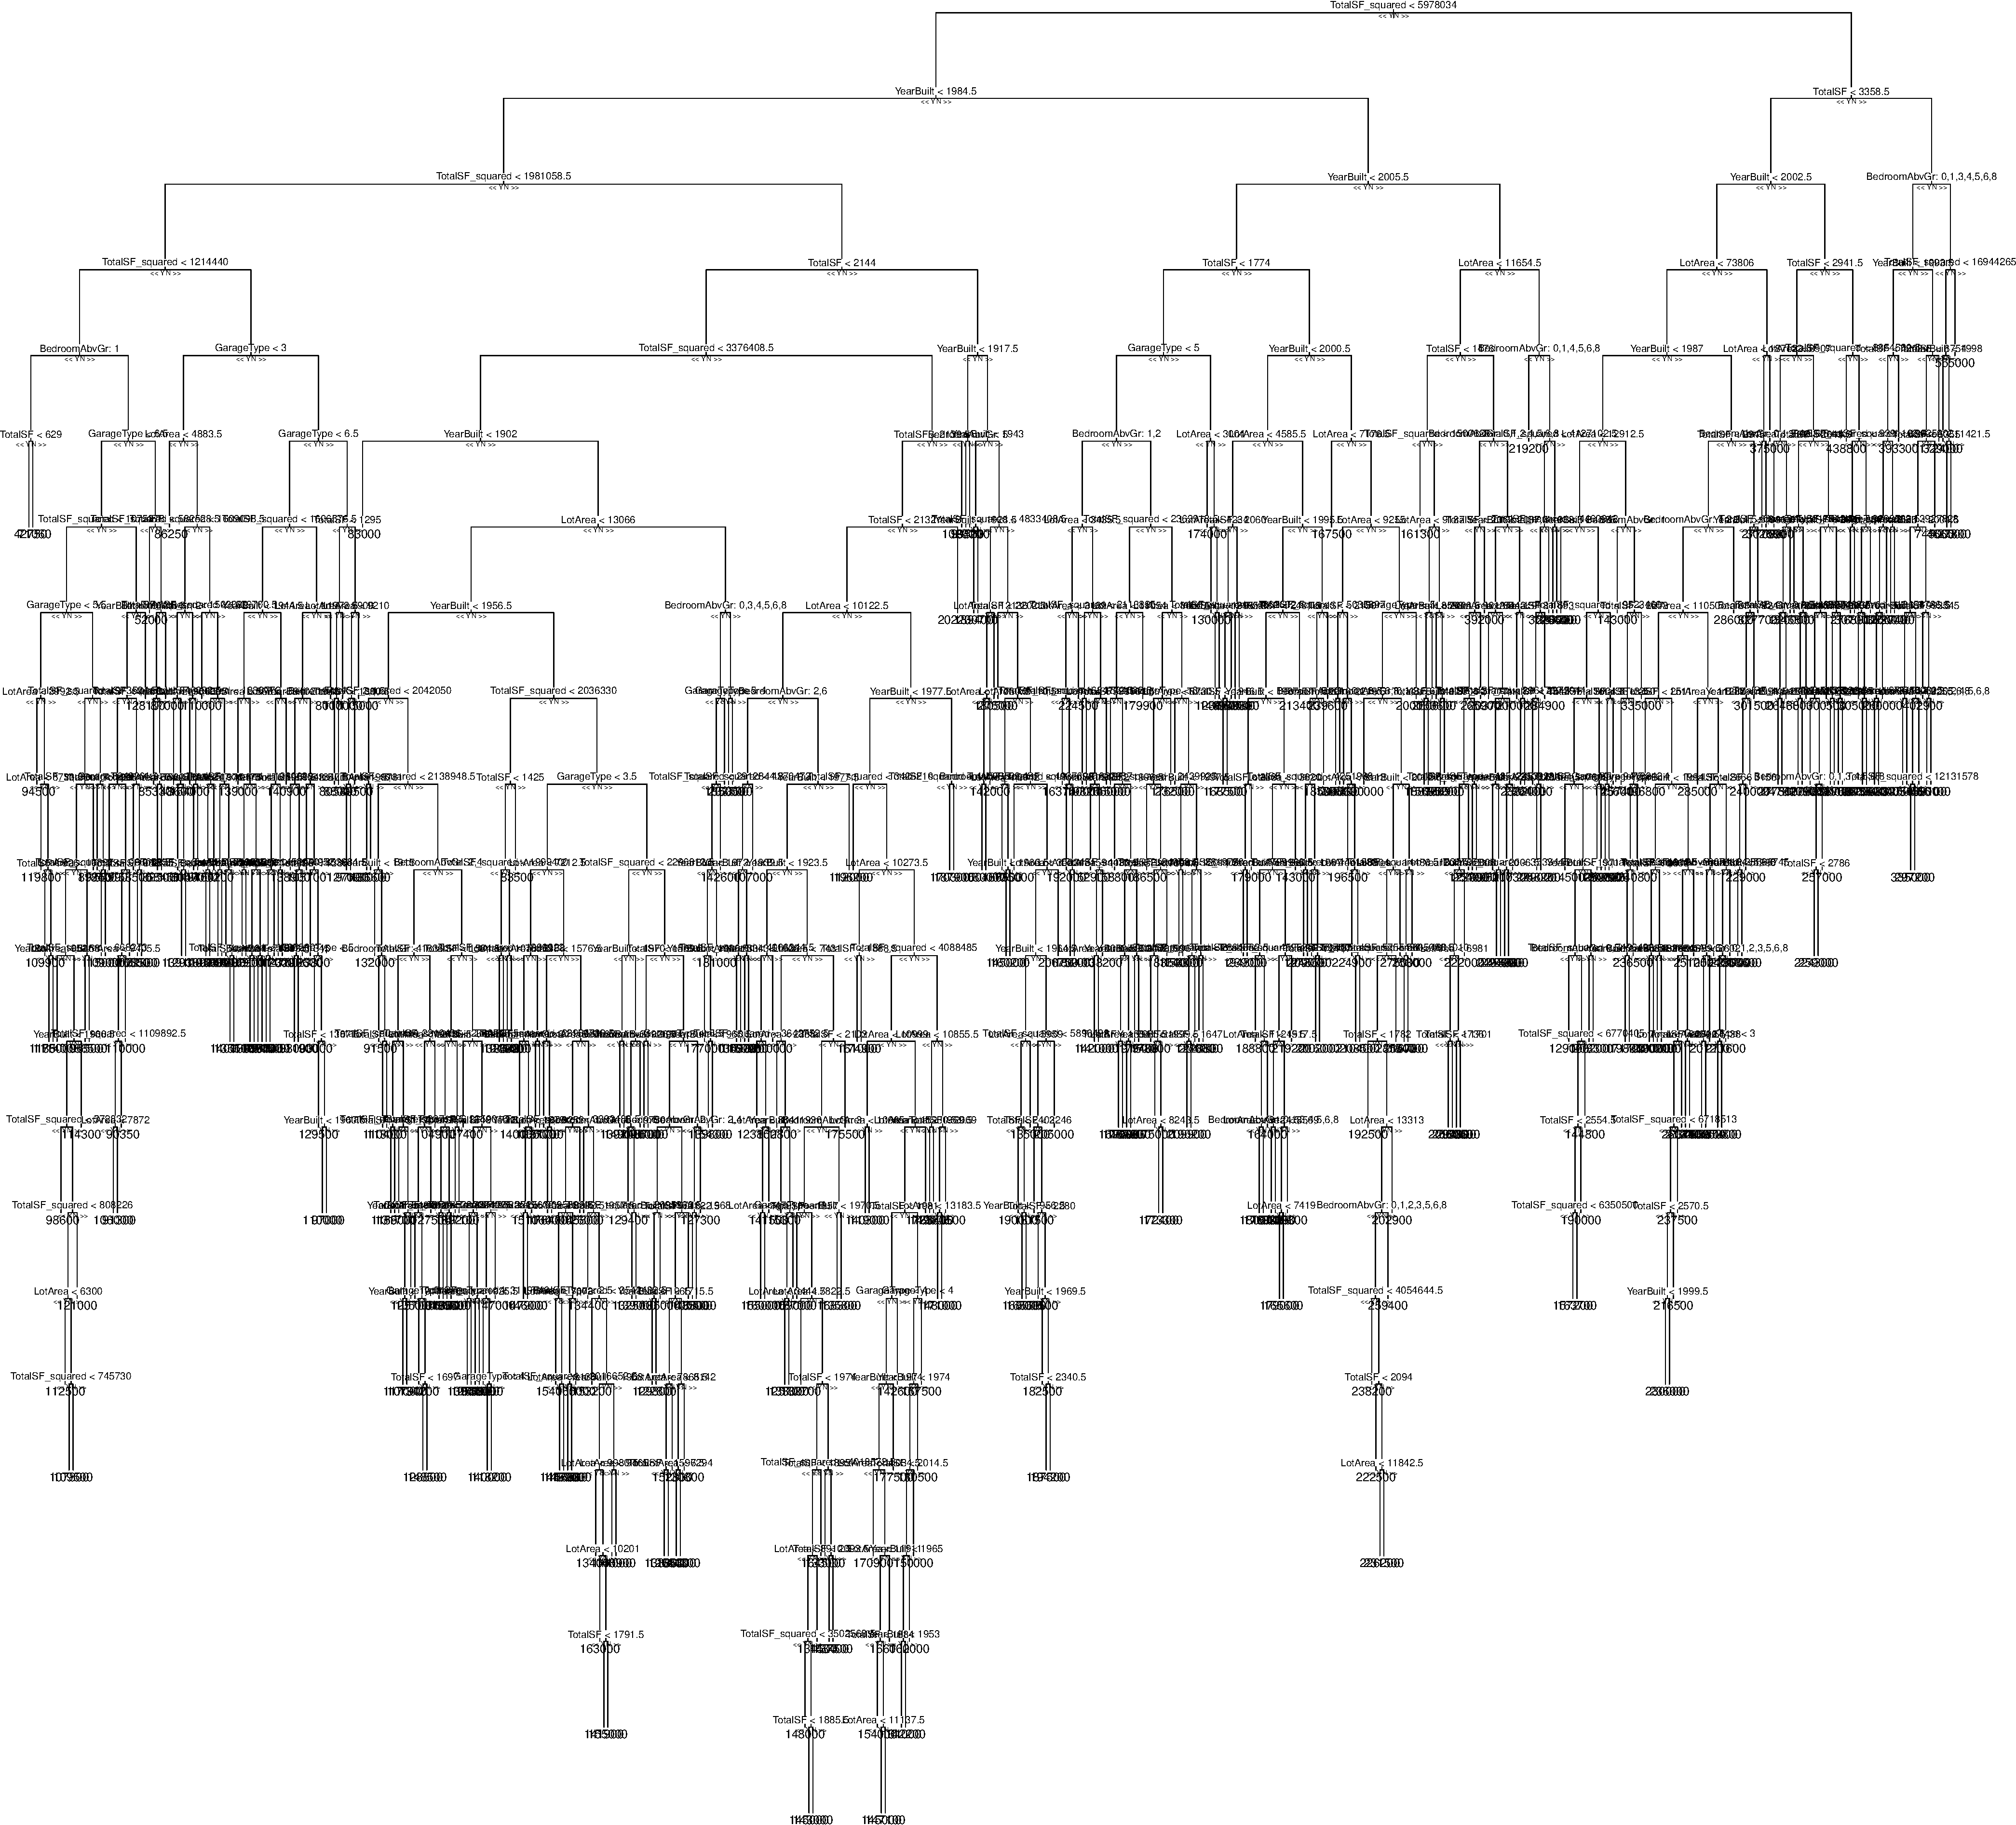
\includegraphics[width=7in,height=7in]{STAT847_W24_Final_files/figure-latex/unnamed-chunk-17-1}

\begin{table}[!h]
\centering
\caption{Evaluation parameters of our Random Forest model}
\begin{tabular}{|c|c|}
\hline
& \textbf{Random Forest Model} \\
\hline
\textbf{RMSE} & 17,356.16 \\
\hline
\textbf{R Squared} & 0.96 \\
\hline
\end{tabular}
\end{table}

\begin{Shaded}
\begin{Highlighting}[]
\FunctionTok{library}\NormalTok{(ggplot2)}
\FunctionTok{ggplot}\NormalTok{(Q4\_df, }\FunctionTok{aes}\NormalTok{(}\AttributeTok{x =}\NormalTok{ SalePrice, }\AttributeTok{y =}\NormalTok{ predictions)) }\SpecialCharTok{+}
    \FunctionTok{geom\_point}\NormalTok{(}\AttributeTok{alpha =} \FloatTok{0.5}\NormalTok{) }\SpecialCharTok{+} \FunctionTok{geom\_smooth}\NormalTok{(}\AttributeTok{method =} \StringTok{"lm"}\NormalTok{,}
    \AttributeTok{color =} \StringTok{"blue"}\NormalTok{) }\SpecialCharTok{+} \FunctionTok{labs}\NormalTok{(}\AttributeTok{title =} \StringTok{"Actual vs. Predicted SalePrice"}\NormalTok{,}
    \AttributeTok{x =} \StringTok{"Actual SalePrice"}\NormalTok{, }\AttributeTok{y =} \StringTok{"Predicted SalePrice"}\NormalTok{)}
\end{Highlighting}
\end{Shaded}

\begin{figure}
\centering
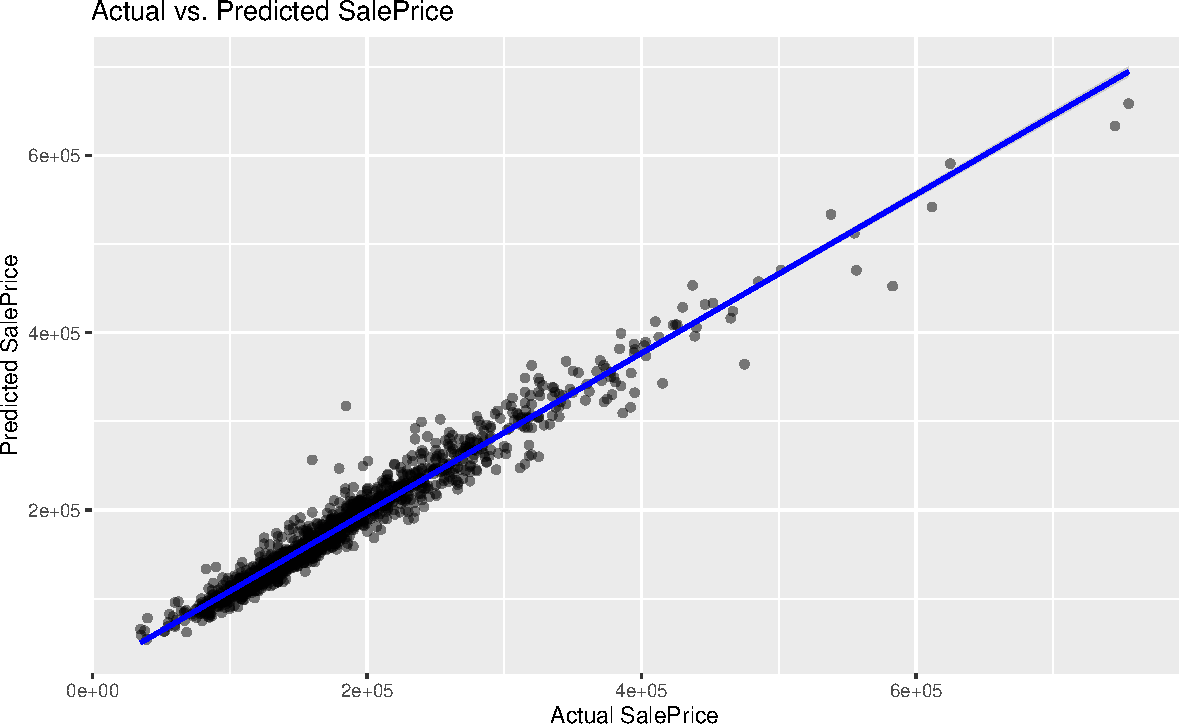
\includegraphics{STAT847_W24_Final_files/figure-latex/unnamed-chunk-19-1.pdf}
\caption{Plot displaying the predicted prices against the actual values
with a blue 45 degree line}
\end{figure}

\newpage

\begin{Shaded}
\begin{Highlighting}[]
\CommentTok{\# Plot t{-}SNE results}
\FunctionTok{plot}\NormalTok{(tsne\_results}\SpecialCharTok{$}\NormalTok{Y[, }\DecValTok{1}\NormalTok{], tsne\_results}\SpecialCharTok{$}\NormalTok{Y[, }\DecValTok{2}\NormalTok{],}
    \AttributeTok{col =}\NormalTok{ Q4\_df}\SpecialCharTok{$}\NormalTok{BldgType, }\AttributeTok{pch =} \DecValTok{19}\NormalTok{, }\AttributeTok{cex =} \FloatTok{0.5}\NormalTok{,}
    \AttributeTok{main =} \StringTok{"t{-}SNE plot"}\NormalTok{)}
\FunctionTok{legend}\NormalTok{(}\StringTok{"topright"}\NormalTok{, }\AttributeTok{legend =} \FunctionTok{levels}\NormalTok{(}\FunctionTok{factor}\NormalTok{(Q4\_df}\SpecialCharTok{$}\NormalTok{BldgType)),}
    \AttributeTok{col =} \DecValTok{1}\SpecialCharTok{:}\FunctionTok{length}\NormalTok{(}\FunctionTok{levels}\NormalTok{(}\FunctionTok{factor}\NormalTok{(Q4\_df}\SpecialCharTok{$}\NormalTok{BldgType))),}
    \AttributeTok{pch =} \DecValTok{19}\NormalTok{)}
\end{Highlighting}
\end{Shaded}

\begin{figure}
\centering
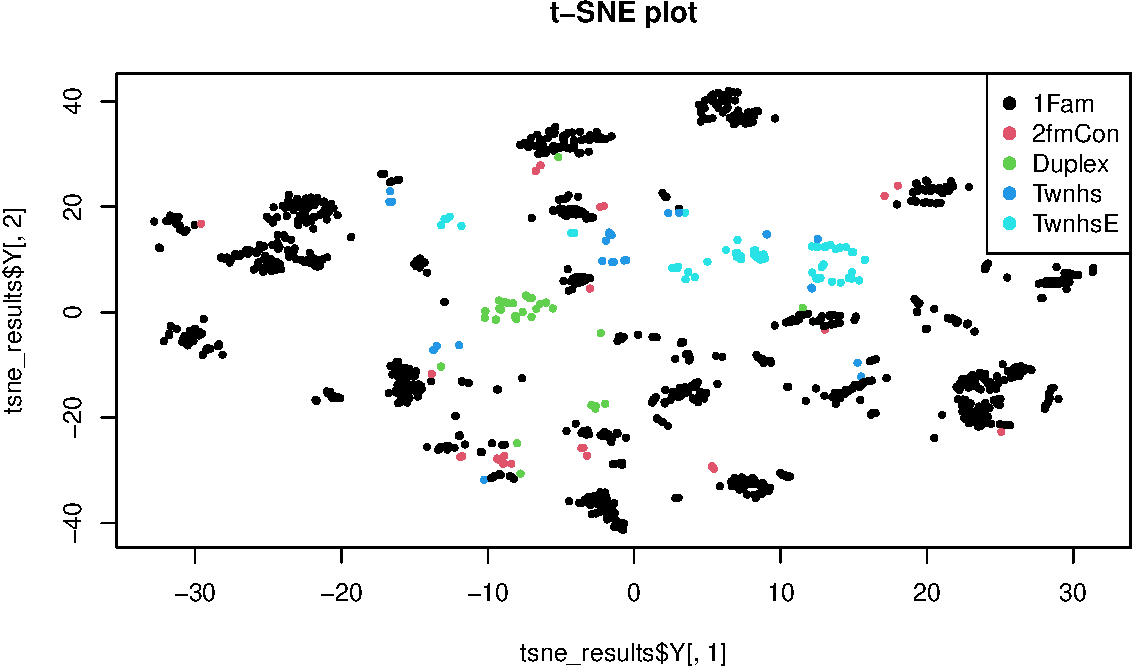
\includegraphics{STAT847_W24_Final_files/figure-latex/unnamed-chunk-22-1.pdf}
\caption{Plot displaying the t-SNE results}
\end{figure}

\newpage

\newpage

\begin{enumerate}
\def\labelenumi{\arabic{enumi})}
\setcounter{enumi}{5}
\tightlist
\item
  \textbf{OPTIONAL: PICK 2 OF 4} Build a visually impressive ggplot to
  show the relationship between at least three variables.
\end{enumerate}

\begin{Shaded}
\begin{Highlighting}[]
\NormalTok{Q4\_df}\SpecialCharTok{$}\NormalTok{BedroomAbvGr }\OtherTok{\textless{}{-}} \FunctionTok{as.factor}\NormalTok{(Q4\_df}\SpecialCharTok{$}\NormalTok{BedroomAbvGr)}
\NormalTok{Q4\_df}\SpecialCharTok{$}\NormalTok{remodel }\OtherTok{\textless{}{-}} \FunctionTok{as.factor}\NormalTok{(Q4\_df}\SpecialCharTok{$}\NormalTok{remodel)}

\FunctionTok{ggplot}\NormalTok{(Q4\_df, }\FunctionTok{aes}\NormalTok{(}\AttributeTok{x =}\NormalTok{ BedroomAbvGr, }\AttributeTok{y =}\NormalTok{ SalePrice,}
    \AttributeTok{color =}\NormalTok{ remodel)) }\SpecialCharTok{+} \FunctionTok{geom\_boxplot}\NormalTok{(}\AttributeTok{outlier.colour =} \StringTok{"black"}\NormalTok{,}
    \AttributeTok{outlier.shape =} \DecValTok{18}\NormalTok{, }\AttributeTok{outlier.size =} \DecValTok{1}\NormalTok{, }\AttributeTok{notch =} \ConstantTok{FALSE}\NormalTok{) }\SpecialCharTok{+}
    \FunctionTok{labs}\NormalTok{(}\AttributeTok{title =} \StringTok{"A boxplot depicting the relationship between Sale Price, Bedrooms and remodel"}\NormalTok{)}
\end{Highlighting}
\end{Shaded}

\begin{figure}
\centering
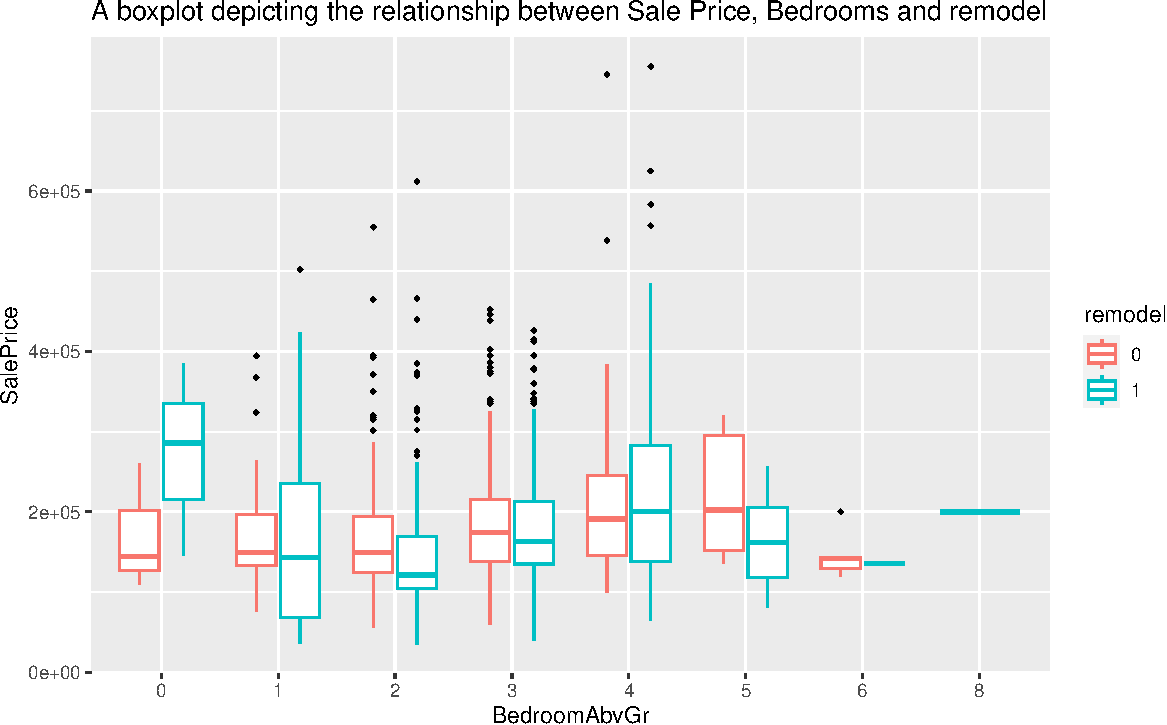
\includegraphics{STAT847_W24_Final_files/figure-latex/unnamed-chunk-25-1.pdf}
\caption{A boxplot depicting the relationship between Sale Price and
Bedrooms above grade with a hue showing whether the home was remodeled
or not}
\end{figure}

\begin{Shaded}
\begin{Highlighting}[]
\FunctionTok{ggplot}\NormalTok{(Q4\_df, }\FunctionTok{aes}\NormalTok{(}\AttributeTok{x =}\NormalTok{ YearBuilt, }\AttributeTok{y =}\NormalTok{ SalePrice,}
    \AttributeTok{color =}\NormalTok{ remodel)) }\SpecialCharTok{+} \FunctionTok{geom\_point}\NormalTok{(}\AttributeTok{size =} \DecValTok{2}\NormalTok{, }\AttributeTok{shape =} \DecValTok{19}\NormalTok{) }\SpecialCharTok{+}
    \FunctionTok{labs}\NormalTok{(}\AttributeTok{title =} \StringTok{"Scatter plot depicting the relationship between Sale Price, YearBuilt and remodel"}\NormalTok{)}
\end{Highlighting}
\end{Shaded}

\begin{figure}
\centering
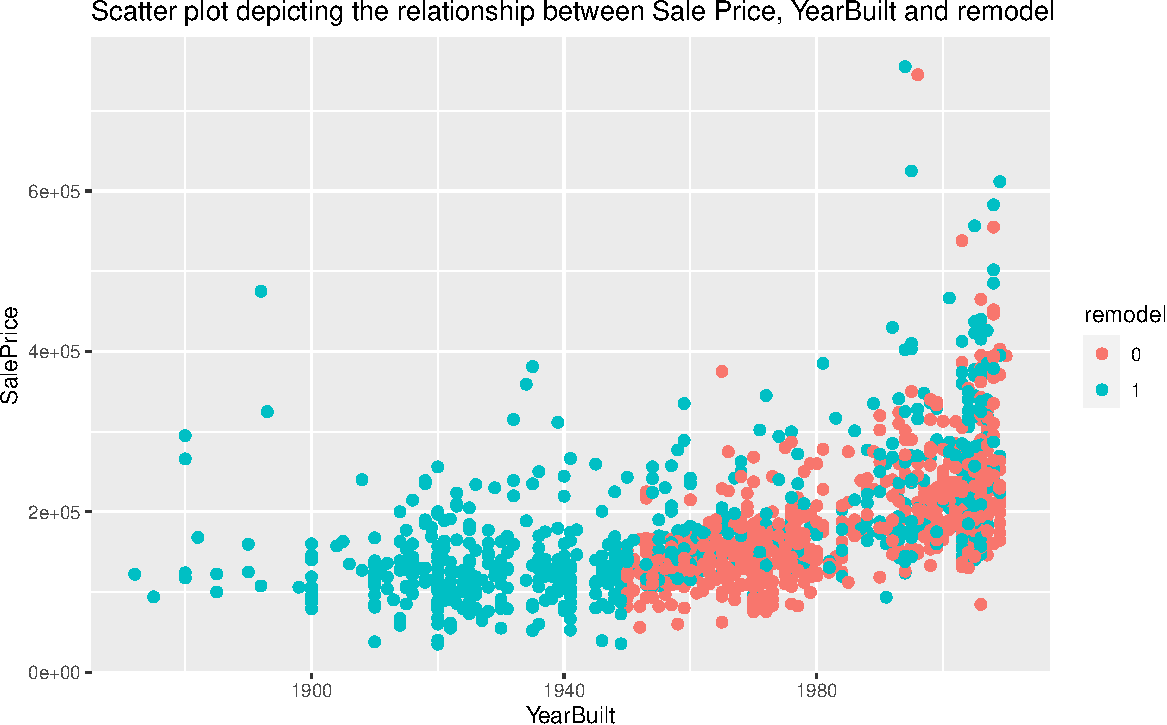
\includegraphics{STAT847_W24_Final_files/figure-latex/unnamed-chunk-26-1.pdf}
\caption{A scatter plot depicting the relationship between Sale Price
and YearBuilt with a hue showing whether the home was remodeled or not}
\end{figure}

\vspace{2cm}

\vspace{2cm}

\newpage

\begin{enumerate}
\def\labelenumi{\arabic{enumi})}
\setcounter{enumi}{7}
\tightlist
\item
  \textbf{OPTIONAL: PICK 2 OF 4} Discuss briefly any ethical concerns
  like residual disclosure that might arise from the use of your data
  set, possibly in combination with some additional data outside your
  dataset.
\end{enumerate}

When working with data it is always crucial to identify potential ethics
concerns that could arise from the data's availability to the public.
The dataset I used for this project is the housing data from Ames
between the years 1872 to 2010, the data is very detailed including
columns for year and month sold, Neighborhood detailing the physical
location within Ames city limits, Proximity to various
conditions(i.e.~Artery Adjacent to arterial street, Feedr Adjacent to
feeder street, Norm Normal, RRNn Within 200' of North-South Railroad),
etc. Firstly this could be a major ethics concern since having all these
details about a home combined with a dataset including home purchases in
the same or other cities or areas could potentially lead to the ability
to identify people and follow them to where they move. Secondly this
dataset also contains data on the types of road access, LotFrontage
which captures the linear feet of street connected to property(0 if
none), Street which captures type of road access to property, and Alley
which captures the type of alley access to the property(NA if none).
Having detailed information on the types of access to a property
combined with the area and price of a home could lead to a homeowner
becoming a target for a potential robbery if the home has a alley
access, which could infer an easier getaway and multiple modes of entry,
and is very large and pricey meaning the owner is most likely wealthy
and would be more likely to be storing expensive items in the home.
Lastly under the condition that you combine this dataset with a dataset
containing all the people who work in the cities using details about the
city like population and density this could potentially lead to people
being able to identify where specific individuals live.

\end{document}
